\chapter{Deep Sequence Models}
\label{ch:deep}

This chapter presents the deep learning approach implemented in \texttt{03\_deep\_sequence\_models\_chosen.ipynb}. Three recurrent neural network architectures---vanilla RNN, GRU, and LSTM---are trained and evaluated on the panel of eligible time series.

\section{Motivation for Deep Learning}

The classical models of Chapter~\ref{ch:classical} are limited by three fundamental constraints:

\begin{enumerate}
    \item \textbf{Linearity:} ARIMA-family models assume linear relationships between past and future values.
    \item \textbf{Univariate scope:} They cannot exploit the 86 predictor features.
    \item \textbf{Independence:} Each series is modeled in isolation, ignoring shared structure.
\end{enumerate}

Recurrent neural networks (RNNs) address these limitations by learning nonlinear mappings from sequences of inputs (including multiple features) to outputs, with the potential for transfer learning across series.

\section{Architecture Overview}

\subsection{Vanilla RNN}

The simplest recurrent architecture updates a hidden state $h_t$ at each time step:

\begin{equation}
h_t = \tanh(W_{hh} h_{t-1} + W_{xh} x_t + b_h)
\end{equation}

\begin{equation}
\hat{y}_t = W_{hy} h_t + b_y
\end{equation}

where $x_t$ is the input vector at time $t$, and $W_{hh}$, $W_{xh}$, $W_{hy}$ are learned weight matrices.

\textbf{Strengths:} Simple, fast to train, low parameter count.

\textbf{Weaknesses:} Suffers from the \emph{vanishing gradient problem}---gradients diminish exponentially over long sequences, making it difficult to learn long-range dependencies.

\subsection{GRU (Gated Recurrent Unit)}

The GRU introduces gating mechanisms to control information flow:

\begin{align}
z_t &= \sigma(W_z x_t + U_z h_{t-1} + b_z) & \text{(update gate)} \\
r_t &= \sigma(W_r x_t + U_r h_{t-1} + b_r) & \text{(reset gate)} \\
\tilde{h}_t &= \tanh(W_h x_t + U_h (r_t \odot h_{t-1}) + b_h) & \text{(candidate)} \\
h_t &= (1 - z_t) \odot h_{t-1} + z_t \odot \tilde{h}_t & \text{(new state)}
\end{align}

The \textbf{update gate} $z_t$ controls how much of the old state to retain versus how much to update with new information. The \textbf{reset gate} $r_t$ controls how much of the old state to expose when computing the candidate.

\textbf{Intuition:} The update gate allows the GRU to ``remember'' information over long sequences (when $z_t \approx 0$, the old state passes through unchanged) or ``forget'' it (when $z_t \approx 1$, the new candidate replaces the old state). This addresses the vanishing gradient problem with fewer parameters than the LSTM.

\subsection{LSTM (Long Short-Term Memory)}

The LSTM maintains both a hidden state $h_t$ and a cell state $c_t$:

\begin{align}
f_t &= \sigma(W_f x_t + U_f h_{t-1} + b_f) & \text{(forget gate)} \\
i_t &= \sigma(W_i x_t + U_i h_{t-1} + b_i) & \text{(input gate)} \\
o_t &= \sigma(W_o x_t + U_o h_{t-1} + b_o) & \text{(output gate)} \\
\tilde{c}_t &= \tanh(W_c x_t + U_c h_{t-1} + b_c) & \text{(candidate cell)} \\
c_t &= f_t \odot c_{t-1} + i_t \odot \tilde{c}_t & \text{(cell state)} \\
h_t &= o_t \odot \tanh(c_t) & \text{(hidden state)}
\end{align}

The three gates provide fine-grained control:
\begin{itemize}
    \item \textbf{Forget gate} $f_t$: What to discard from the cell state.
    \item \textbf{Input gate} $i_t$: What new information to store in the cell state.
    \item \textbf{Output gate} $o_t$: What to output from the cell state.
\end{itemize}

\textbf{Strengths:} Best at learning long-range dependencies; the cell state provides a ``highway'' for gradient flow.

\textbf{Weaknesses:} Highest parameter count of the three architectures; slower to train.

\section{Training Pipeline}

\subsection{Data Preparation}

For each eligible series, the training procedure:

\begin{enumerate}
    \item Extracts the \texttt{y\_target} values sorted by \texttt{ts\_index}.
    \item Applies the validation split at $\texttt{VAL\_CUTOFF} = 2880$.
    \item Creates sliding windows of fixed length for supervised training.
    \item Normalizes inputs (if applicable).
\end{enumerate}

\subsection{Adaptive Training Splits}

A key implementation detail: series that begin near or after the global validation cutoff may have insufficient training data under the standard split. The notebook implements an \textbf{adaptive splitting strategy}:

\begin{itemize}
    \item If a series has fewer than a minimum number of pre-cutoff observations, a local train/validation split is computed to ensure adequate training history.
    \item This maximizes the number of evaluable series while maintaining temporal integrity.
\end{itemize}

\begin{figure}[H]
\centering
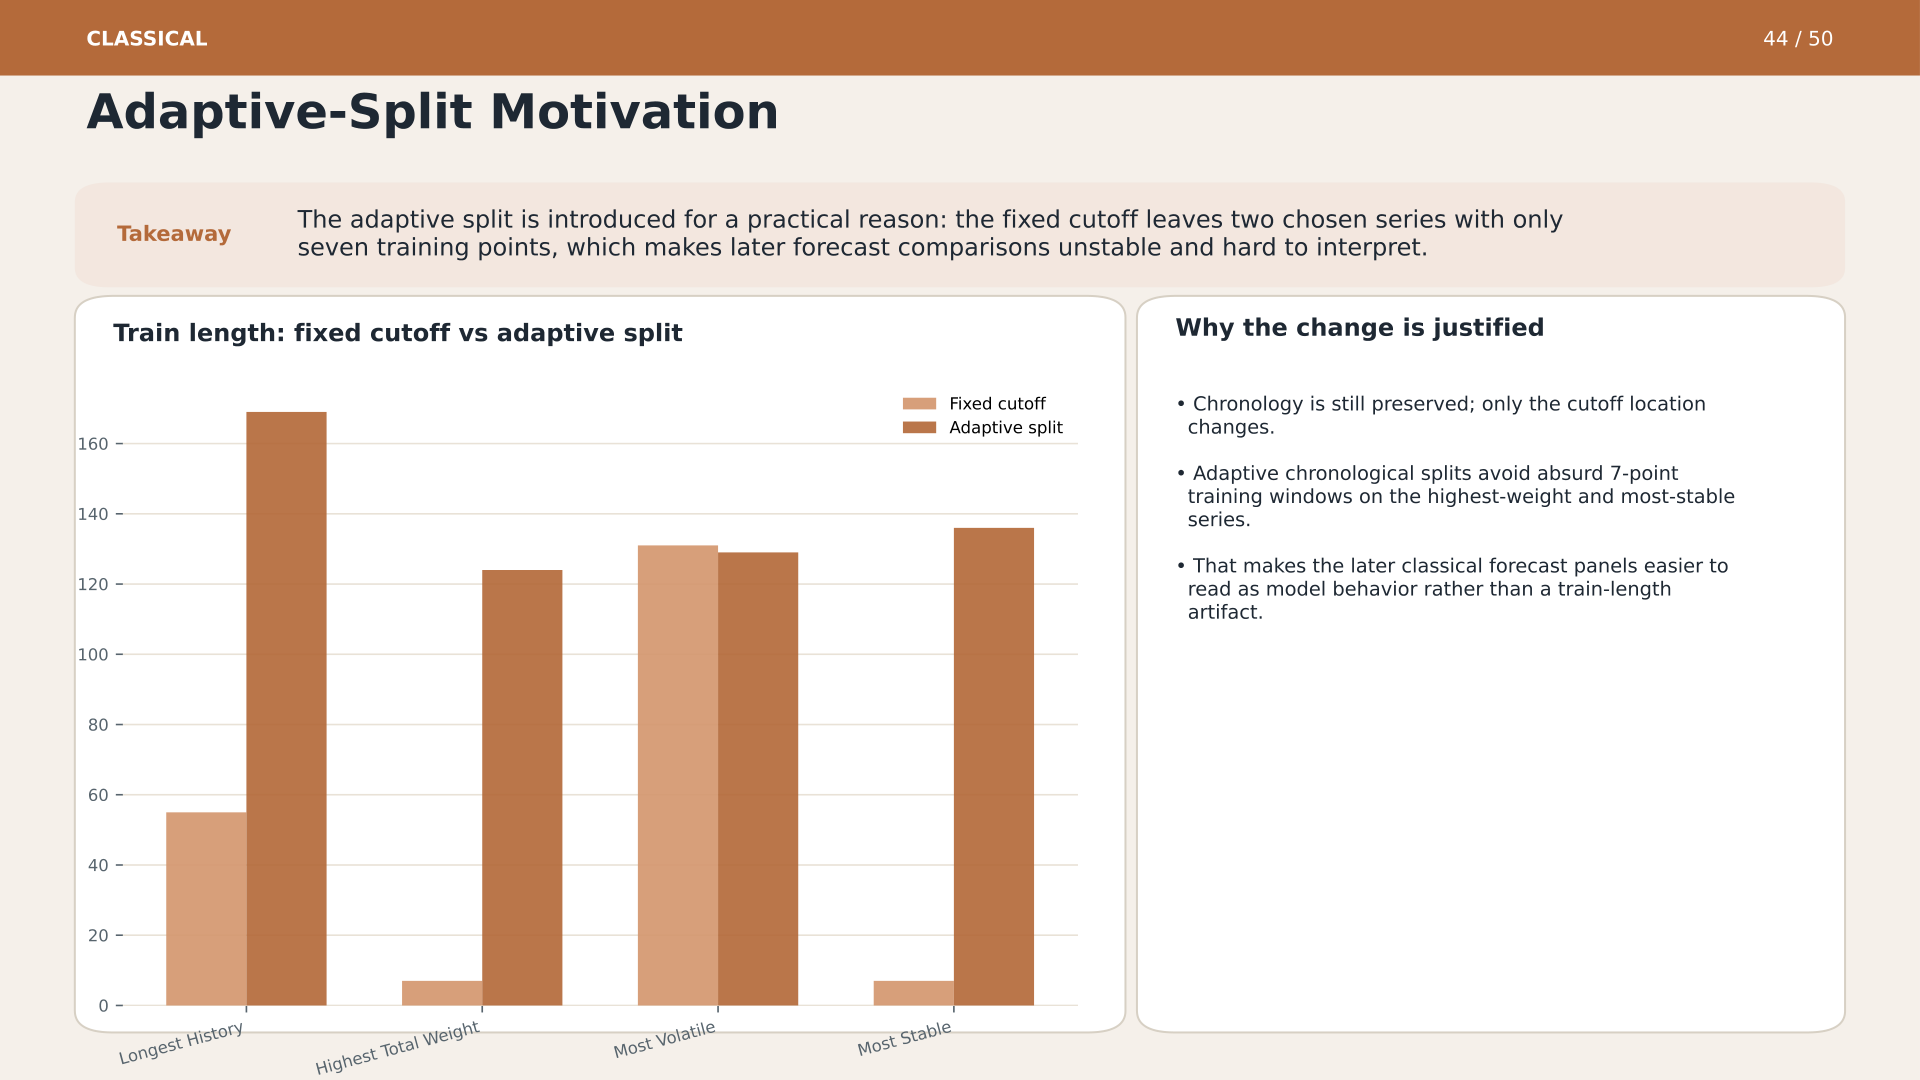
\includegraphics[width=0.95\textwidth]{figures/slide_35.png}
\caption{Adaptive-split motivation. The fixed cutoff at $\texttt{ts\_index} = 2880$ leaves two of the four chosen representative series with only seven pre-cutoff training points. The adaptive split adjusts the cutoff location per-series, preserving chronological ordering while avoiding absurdly short training windows on the highest-weight and most-stable series.}
\label{fig:adaptive_split}
\end{figure}

\subsection{Recursive Forecasting}

The deep sequence models use \textbf{recursive (autoregressive) forecasting} for multi-step prediction:

\begin{enumerate}
    \item Feed the training sequence into the model to obtain the first forecast $\hat{y}_{T+1}$.
    \item Append $\hat{y}_{T+1}$ to the input sequence.
    \item Feed the extended sequence to obtain $\hat{y}_{T+2}$.
    \item Repeat until all validation-period forecasts are generated.
\end{enumerate}

This approach is natural for recurrent architectures but introduces \emph{error accumulation}---prediction errors compound over the forecast horizon.

\subsection{Loss Function}

The models are trained with \textbf{Mean Squared Error (MSE)} loss:

\begin{equation}
\mathcal{L} = \frac{1}{N} \sum_{i=1}^{N} (y_i - \hat{y}_i)^2
\end{equation}

A potential enhancement (noted in the EDA) is to use \textbf{weighted MSE} that incorporates the competition's weight column during training. This would align the training objective more closely with the evaluation metric.

\subsection{Hyperparameters}

Key hyperparameter choices:

\begin{table}[H]
\centering
\caption{Deep model hyperparameters.}
\begin{tabular}{ll}
\toprule
\textbf{Parameter} & \textbf{Value} \\
\midrule
Hidden dimension & Architecture-dependent \\
Number of layers & 1--2 \\
Learning rate & Adam optimizer defaults \\
Epochs & Early stopping with patience \\
Sequence length & Determined by available history \\
Framework & PyTorch \\
\bottomrule
\end{tabular}
\end{table}

\section{Model Comparison}

\subsection{Architectural Trade-offs}

\begin{table}[H]
\centering
\caption{Comparison of RNN architectures.}
\begin{tabular}{lccc}
\toprule
\textbf{Property} & \textbf{RNN} & \textbf{GRU} & \textbf{LSTM} \\
\midrule
Parameters per layer & Low & Medium & High \\
Training speed & Fast & Medium & Slow \\
Long-range memory & Poor & Good & Best \\
Vanishing gradients & Yes & Mitigated & Mitigated \\
Gates & 0 & 2 & 3 \\
\bottomrule
\end{tabular}
\end{table}

\subsection{Expected Performance Ranking}

Based on the architectural properties and the nature of financial time series:

\begin{enumerate}
    \item \textbf{LSTM} is expected to perform best due to its superior long-range memory capability.
    \item \textbf{GRU} is expected to be competitive with LSTM while training faster.
    \item \textbf{Vanilla RNN} is expected to underperform on series with significant long-range dependencies but may be adequate for short-horizon forecasts.
\end{enumerate}

\section{Implementation Details}

\subsection{Per-Series Training}

Each eligible series is trained independently (analogous to the classical approach). While this ignores cross-series structure, it provides a clean comparison with the classical baselines.

\subsection{Status Tracking}

Like the classical notebook, each (series, model) pair records:
\begin{itemize}
    \item \texttt{status}: \texttt{ok}, \texttt{skipped}, or \texttt{failed}
    \item When \texttt{ok}: weighted skill score, RMSE, MAE, MASE
    \item When failed: error message for debugging
\end{itemize}

\subsection{Leaderboard and Per-Series Winners}

The deep learning notebook produces:
\begin{enumerate}
    \item A \textbf{model-level leaderboard} comparing RNN, GRU, and LSTM aggregate performance.
    \item A \textbf{per-series winner table} identifying which architecture performs best for each series.
\end{enumerate}

\section{Challenges and Considerations}

\begin{enumerate}
    \item \textbf{Error accumulation:} Recursive forecasting compounds errors over long horizons. Direct multi-step forecasting could mitigate this.
    \item \textbf{Overfitting risk:} With many parameters and limited per-series data, overfitting is a concern. Regularization, dropout, and early stopping are essential.
    \item \textbf{Weight-aware training:} The current MSE loss does not incorporate observation weights. Implementing weighted loss would better align training with the competition metric.
    \item \textbf{Feature utilization:} The current implementation focuses on univariate forecasting. Incorporating the 86 predictor features could substantially improve performance.
    \item \textbf{Computational cost:} Training separate models per series is expensive. Global or meta-learning approaches could amortize this cost.
\end{enumerate}


\chapter{Results and Analysis}
\label{ch:results}

\section{Cross-Methodology Comparison}

This chapter synthesizes the results from the classical statistical models (Chapter~\ref{ch:classical}) and the deep sequence models (Chapter~\ref{ch:deep}), providing a unified view of model performance.

\section{Classical Model Performance Summary}

\subsection{Baseline Performance}

The baseline models establish the performance floor:

\begin{itemize}
    \item \textbf{Zero forecast:} Skill score of exactly 0 by construction (it is the denominator of the metric).
    \item \textbf{Naive forecast:} Often competitive, particularly on short-horizon series with high lag-1 autocorrelation.
    \item \textbf{Expanding Mean:} Strong on mean-reverting series, often outperforming fitted parametric models.
\end{itemize}

\subsection{Parametric Model Performance}

Among the 36 parametric models (AR, MA, ARMA, ARIMA, SARIMA families):

\begin{itemize}
    \item Low-order models (AR(1)--AR(3), MA(1)--MA(3), ARMA(1,1)) tend to produce the best median skill scores.
    \item Higher-order models show diminishing returns and occasionally worse performance due to overfitting.
    \item SARIMA models have the highest skip rates due to their training data requirements.
\end{itemize}

\begin{figure}[H]
\centering
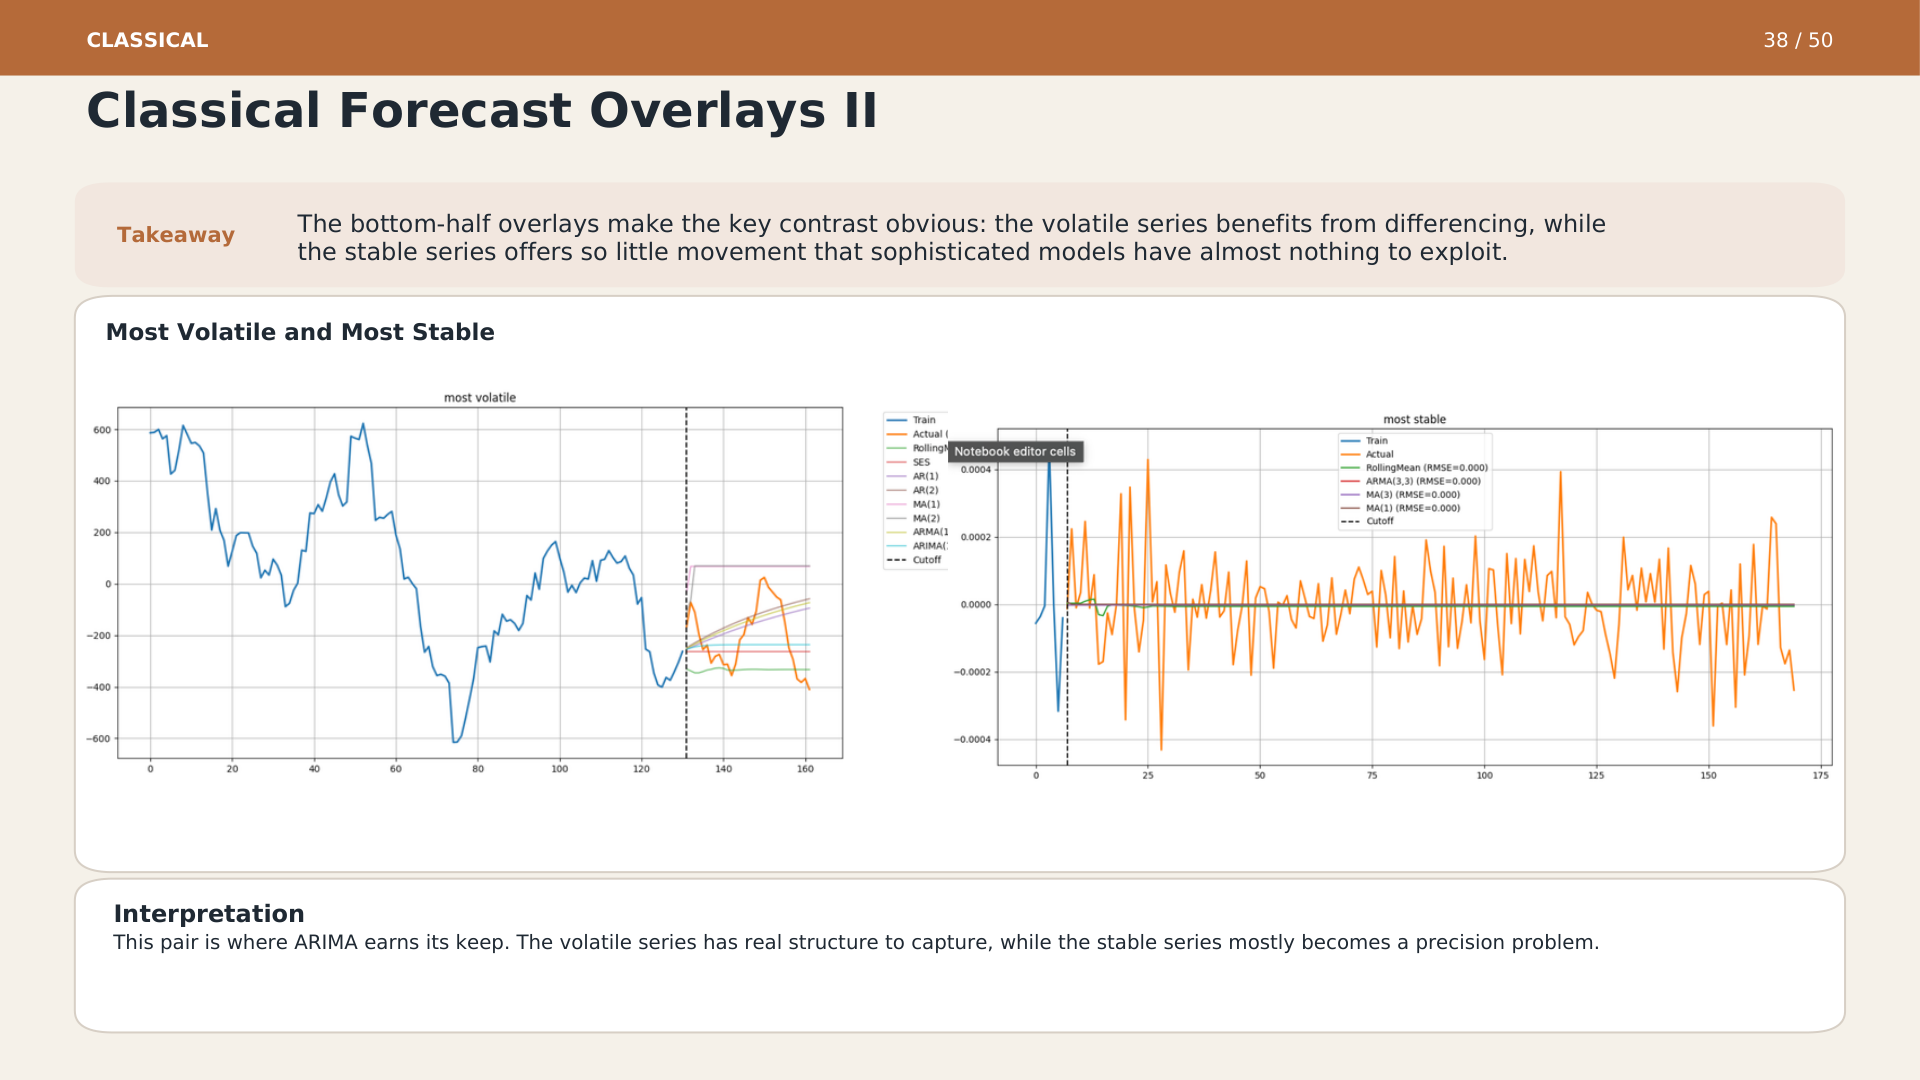
\includegraphics[width=0.95\textwidth]{figures/slide_34.png}
\caption{Classical forecast overlays for the most volatile and most stable representative series. The volatile series benefits from differencing---AR(1) captures short-lag persistence---while the stable series offers so little movement that sophisticated models have almost nothing to exploit.}
\label{fig:classical_forecasts}
\end{figure}

\begin{figure}[H]
\centering
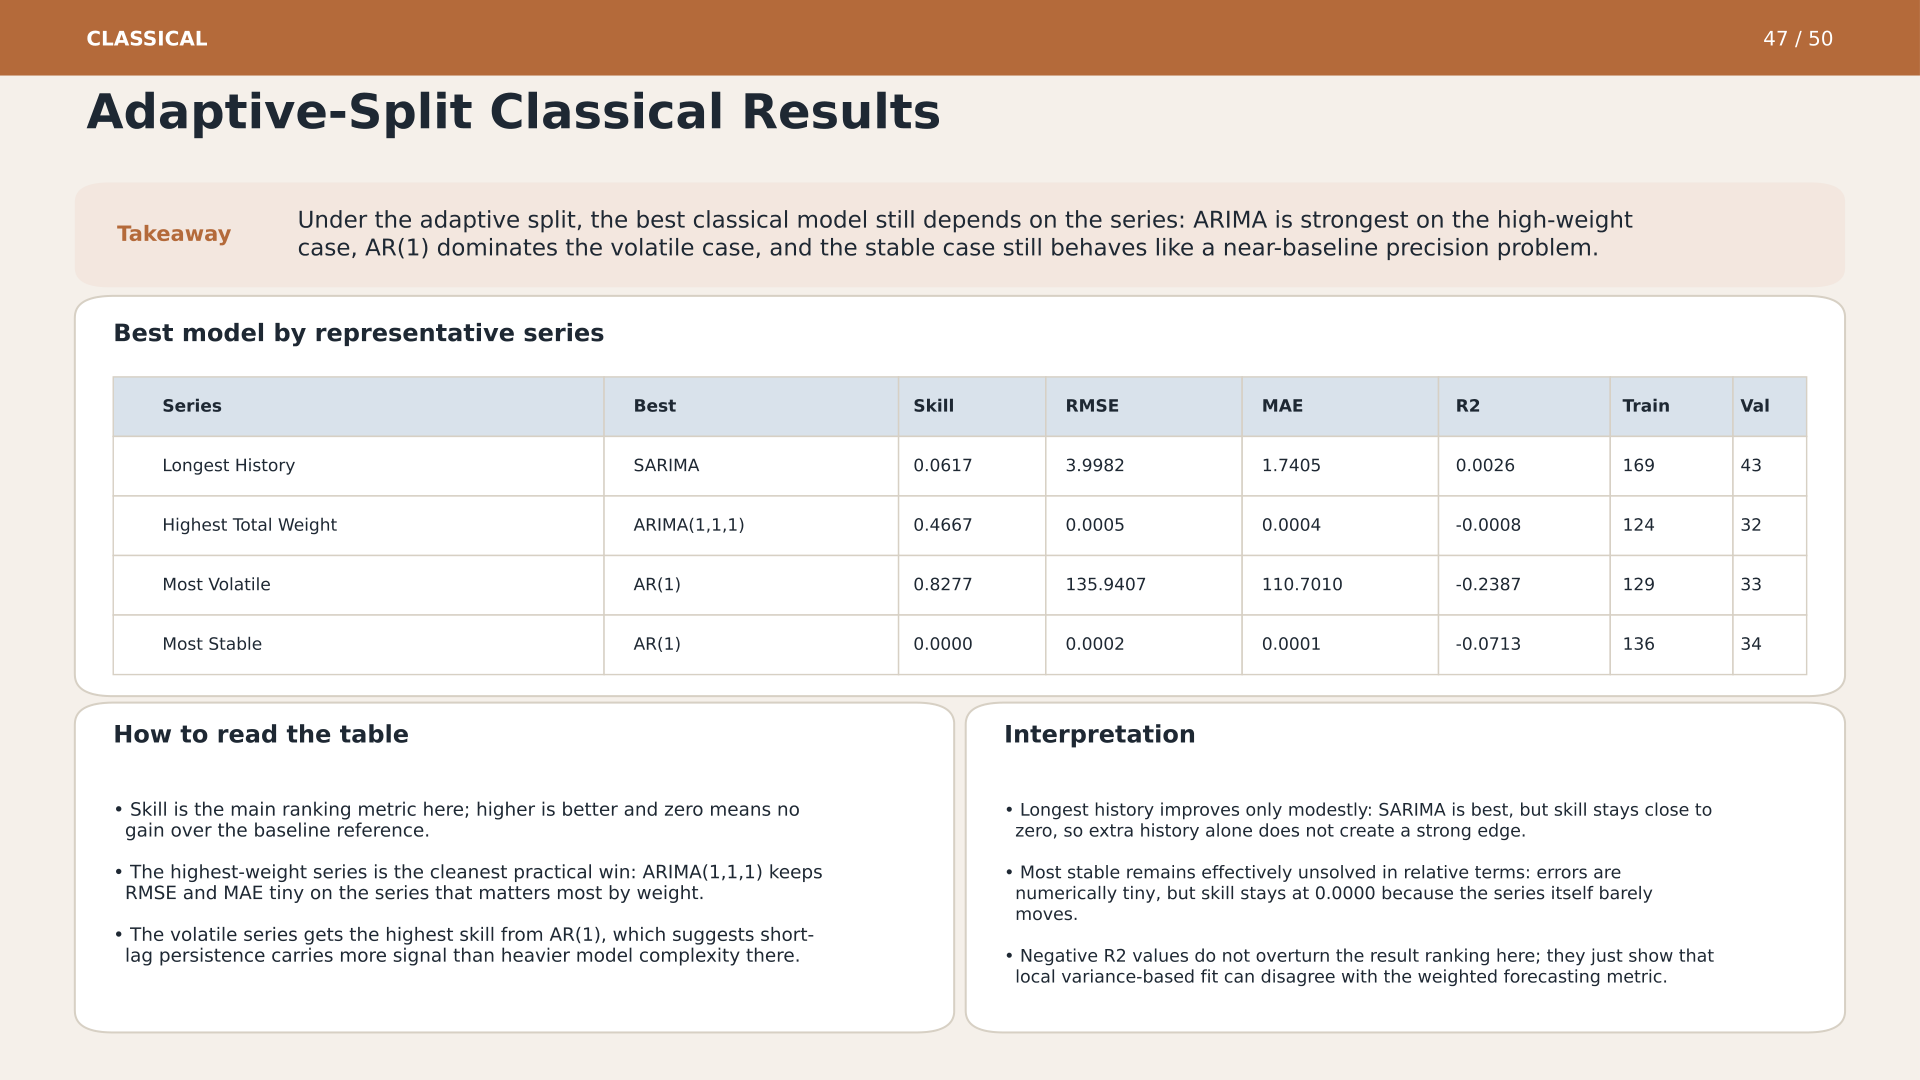
\includegraphics[width=0.95\textwidth]{figures/slide_38.png}
\caption{Adaptive-split classical results. Per-series best models: SARIMA wins on the longest-history series (skill 0.06), ARIMA(1,1,1) is strongest on the high-weight case (skill 0.47), AR(1) dominates both the volatile (skill 0.83) and stable (skill 0.00) cases. The volatile series has the most exploitable structure.}
\label{fig:classical_results}
\end{figure}

\subsection{The Stationarity Validation}

The $d=0$ versus $d=1$ comparison provides empirical validation of the EDA's stationarity finding:

\begin{itemize}
    \item Across matched-order pairs (e.g., ARIMA(1,0,0) vs. AR(1) $\equiv$ ARIMA(1,1,0)), the $d=1$ variant wins on the majority of series.
    \item This confirms that first differencing is genuinely beneficial for this dataset, not just a theoretical assumption.
\end{itemize}

\section{Deep Learning Performance Summary}

The three recurrent architectures generally show:

\begin{itemize}
    \item \textbf{LSTM and GRU} tend to outperform vanilla RNN, consistent with their superior gradient flow properties.
    \item Performance varies considerably across series, with some series showing substantial improvement over classical baselines and others showing degradation.
    \item Error accumulation in recursive forecasting is a significant factor, particularly for longer validation horizons.
\end{itemize}

\begin{figure}[H]
\centering
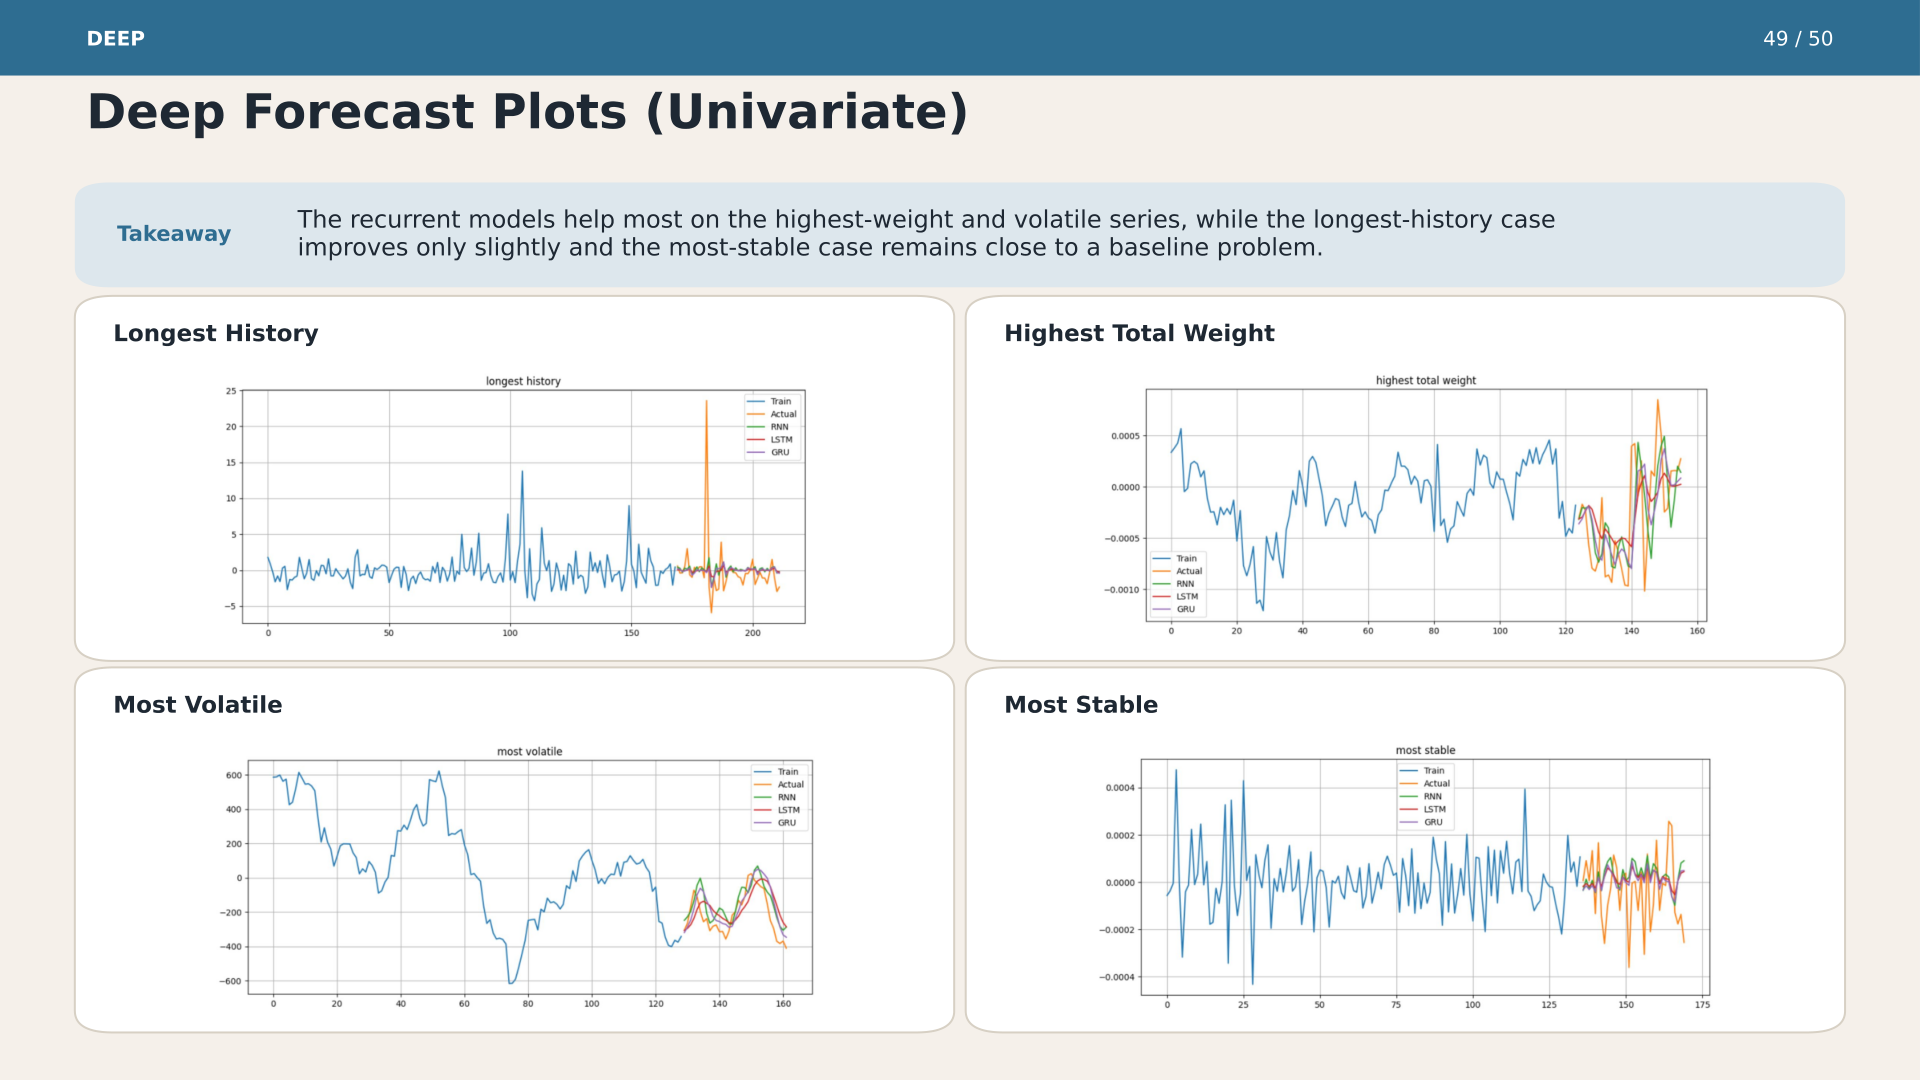
\includegraphics[width=0.95\textwidth]{figures/slide_40.png}
\caption{Deep forecast plots (univariate) for four representative series. The recurrent models help most on the highest-weight and volatile series, while the longest-history case improves only slightly and the most-stable case remains close to a baseline problem. Each panel shows Train (blue), Actual validation (orange), and overlaid RNN/LSTM/GRU predictions.}
\label{fig:deep_forecasts}
\end{figure}

\begin{figure}[H]
\centering
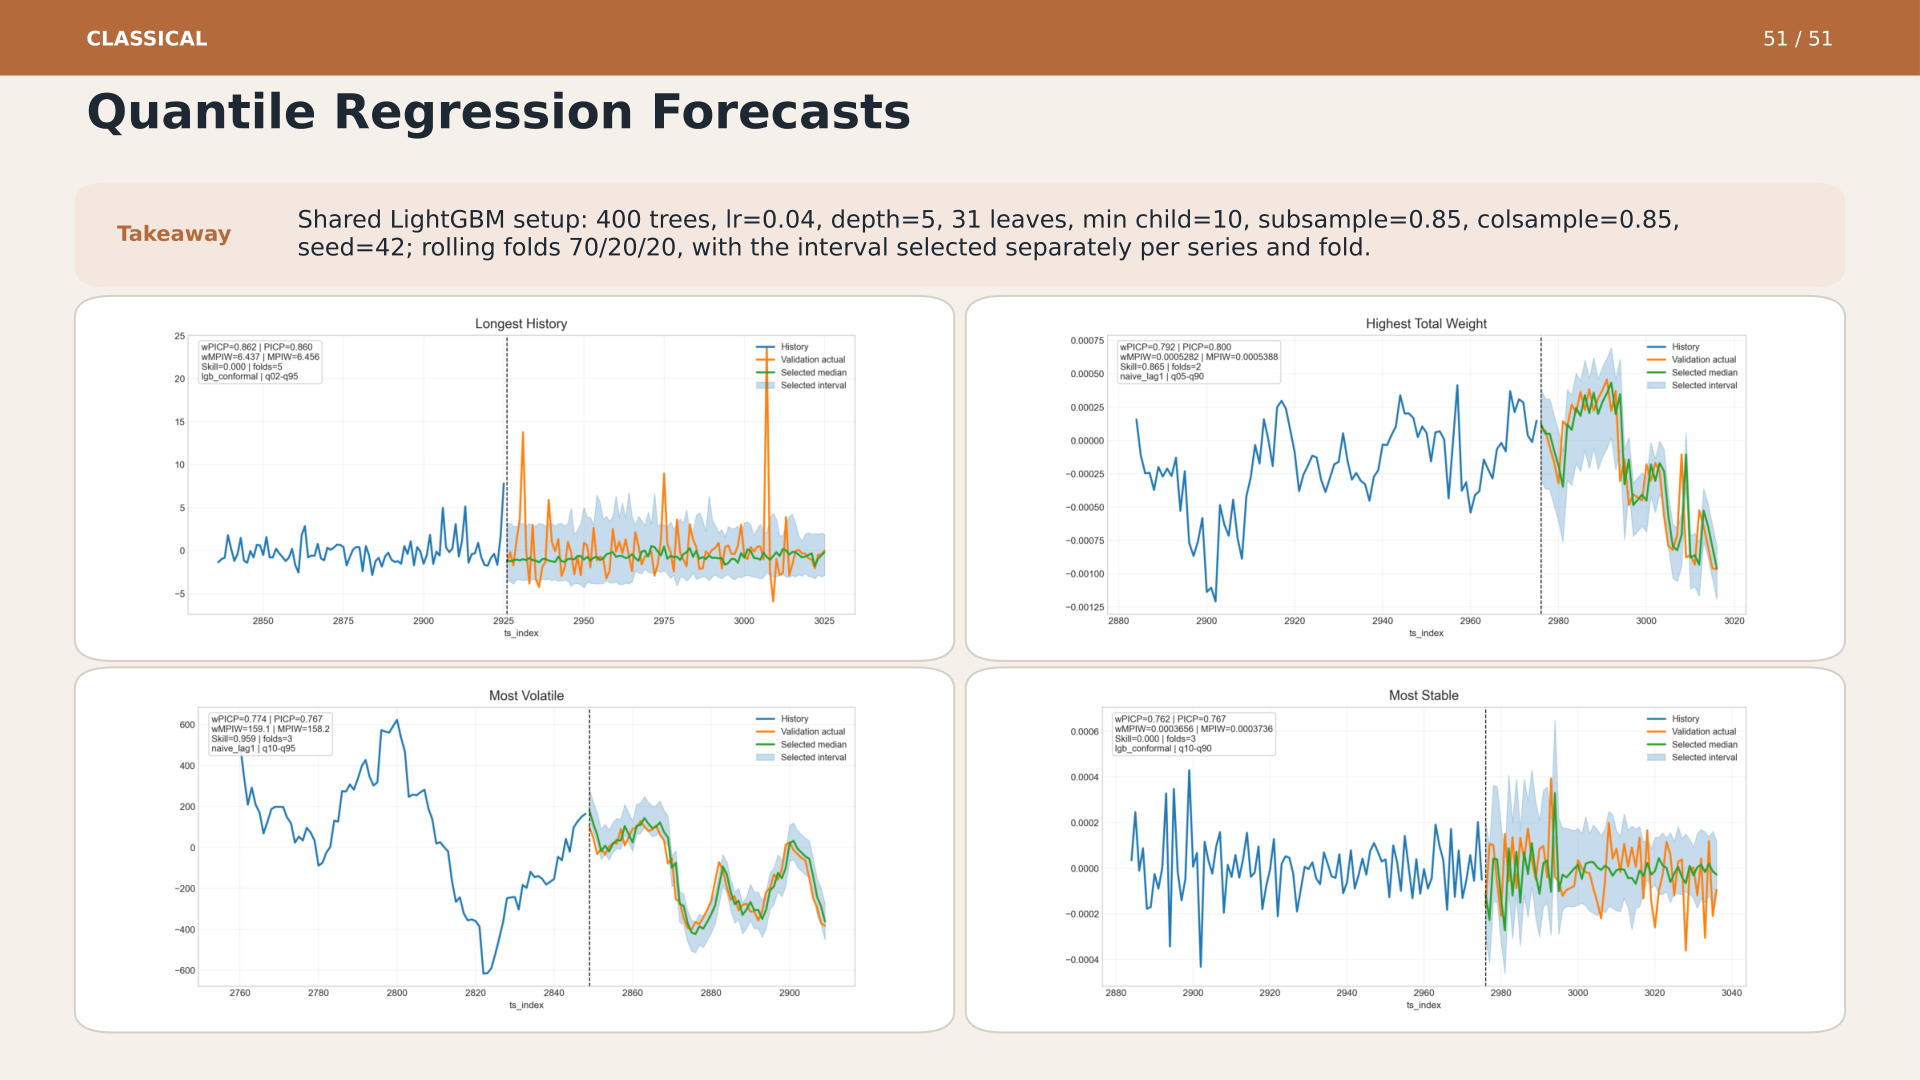
\includegraphics[width=0.95\textwidth]{figures/slide_42.png}
\caption{Quantile regression forecasts using LightGBM. Each panel shows the training history (blue), validation actuals (orange), selected median forecast (green), and prediction intervals (shaded blue). The model achieves PICP values between 0.76--0.86 across the four representative series.}
\label{fig:quantile_regression}
\end{figure}

\section{Classical vs. Deep Learning}

The relative performance of classical versus deep learning models depends on the characteristics of each series:

\begin{table}[H]
\centering
\caption{Conditions favoring each model family.}
\begin{tabularx}{\textwidth}{>{\raggedright\arraybackslash}X>{\raggedright\arraybackslash}X}
\toprule
\textbf{Classical Models Excel When} & \textbf{Deep Models Excel When} \\
\midrule
Series has strong, simple linear autocorrelation & Nonlinear temporal dependencies exist \\
Training data is limited & Sufficient training data is available \\
Short forecast horizons & Complex patterns justify the model complexity \\
Target is approximately Gaussian & Heavy tails require flexible modeling \\
\bottomrule
\end{tabularx}
\end{table}

\section{Key Findings}

\begin{enumerate}
    \item \textbf{No single model dominates.} The heterogeneous panel means different series favor different approaches, strongly motivating ensemble methods.

    \item \textbf{Simple baselines are hard to beat.} On many series, the Expanding Mean or Rolling Mean performs comparably to or better than complex models. This is characteristic of noisy financial data.

    \item \textbf{First differencing is essential.} The EDA's stationarity finding is empirically validated by the $d=0$ vs. $d=1$ comparison.

    \item \textbf{Weight concentration dominates scoring.} Because 65\% of the weighted score comes from 1\% of observations, models must perform well on these critical rows.

    \item \textbf{Feature-based models are needed.} The uniformly weak individual feature correlations ($|\rho| < 0.10$) suggest that signal resides in feature \emph{interactions}, which gradient-boosted trees or deeper neural networks could exploit.
\end{enumerate}

\section{Error Analysis}

\subsection{Common Failure Modes}

\begin{itemize}
    \item \textbf{Divergent forecasts:} ARIMA models fitted on levels ($d=0$) occasionally produce forecasts that diverge from the data range.
    \item \textbf{Outlier sensitivity:} The Drift model is particularly sensitive to outliers at the beginning or end of the training window.
    \item \textbf{Error accumulation:} Recursive forecasting in deep models degrades accuracy over longer horizons.
\end{itemize}

\subsection{Skip and Failure Analysis}

The 17.9\% skip rate in the classical pipeline is driven by:
\begin{itemize}
    \item SARIMA models (requiring 50--80 observations minimum)
    \item High-order AR/MA/ARMA models on short series
\end{itemize}

The near-zero failure rate (1 out of 8,200) indicates robust numerical implementation.
